%-------------------------------------------------
% FileName: chap-5.tex
% Description: 第5章 系统详细设计与实现
%-------------------------------------------------

\chapter{系统详细设计与实现}

\section{场地列表与筛选实现}

场地列表页是普通用户进入到系统以后的最主要的一个入口。页面上没有使用复杂的查询条件，仅保留了场地类型的筛选以及分页浏览，因为体育馆场地数量比较少，一般用户都会先根据运动项目来查找，再按照开放时间与价格决定是否预约。前端在 VenueList.vue 中调用 /api/venues 接口，请求参数包括页码、每页数量和可选的 type。接口返回之后，页面会显示场地名称、类型、开放时间、单价以及状态，并且把“预约”按钮放在每个场地条目旁边。

后端查询逻辑在场地相关接口中进行。系统将所有位于上架位置的场地都对普通用户开放预约权限，管理员可于后台查询全部的场地信息，并可对它们的状态进行调节。这样处理之后，场地临时维修或者停止对外开放的时候，不需要删除数据，只需要把状态改为下架即可。数据库中保存着这个场地历史订单记录，之后统计或者追溯的时候不会丢失。

\begin{figure}[htbp]
\centering
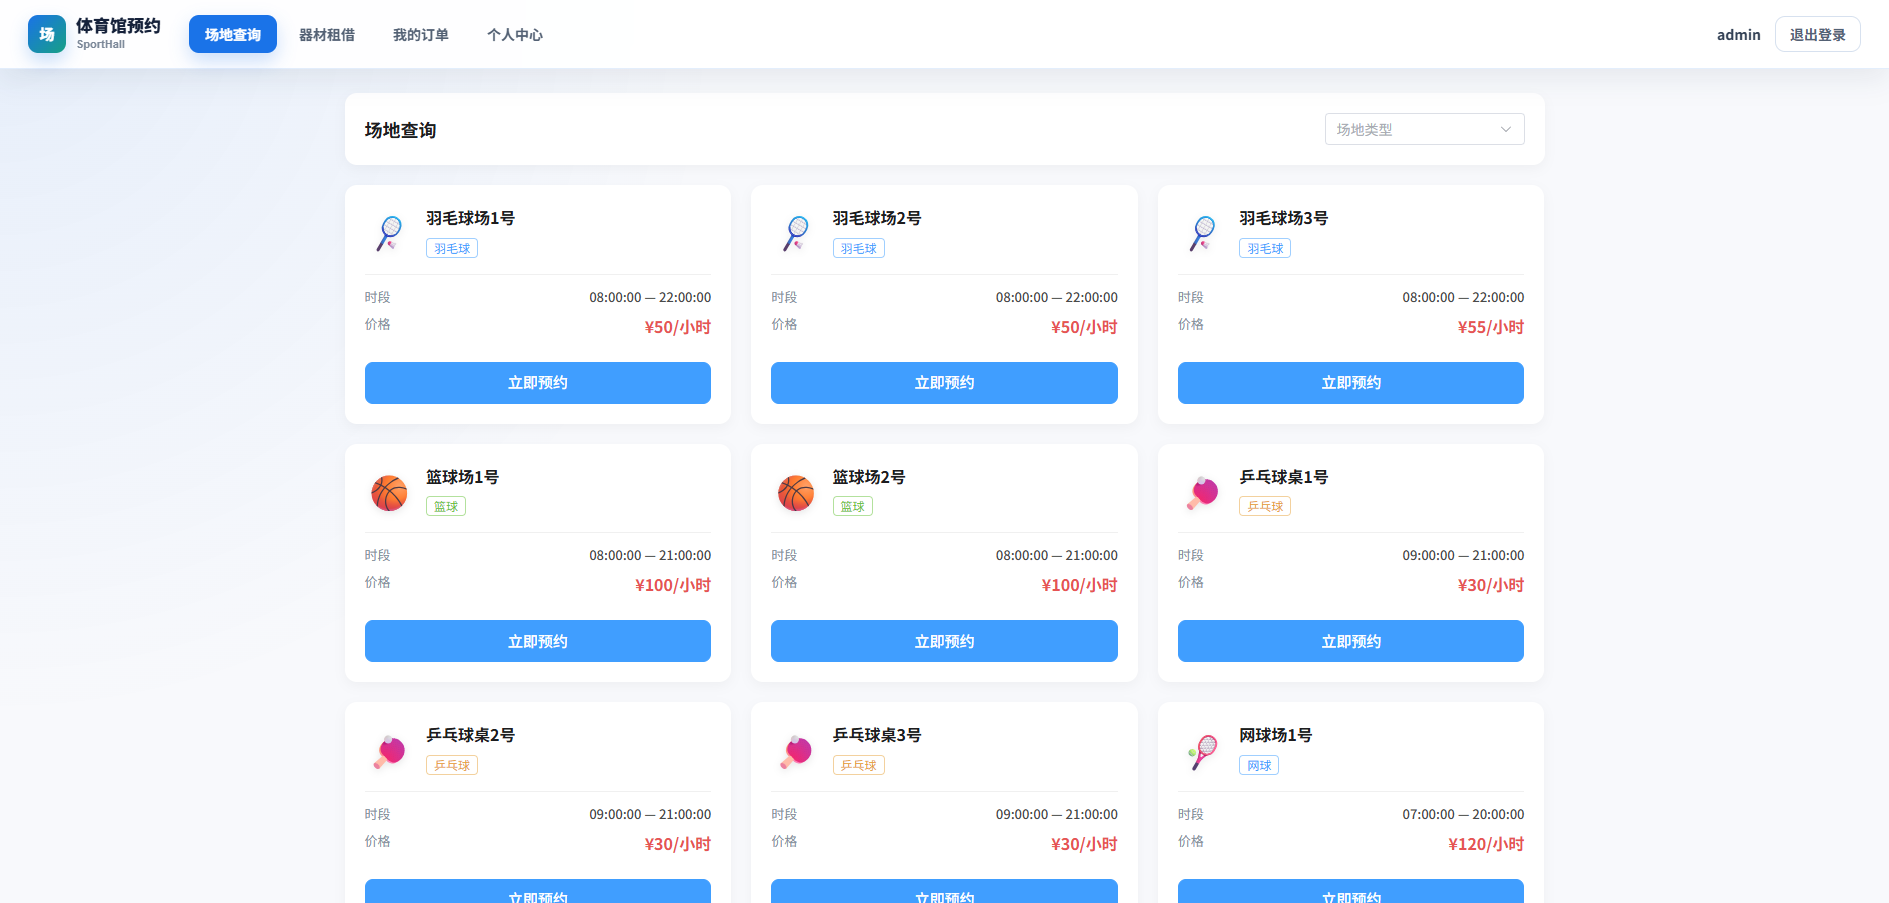
\includegraphics[width=0.8\textwidth]{img/fig5-1.png}
\caption{场地列表与筛选页面}
\label{fig:venue-list-ui}
\end{figure}

\section{预约时段选择与下单实现}

预约页面的主要功能就是“先让用户看到哪些时间不能选”。用户在场地列表页面中到达预约页时，前端会根据路由中的场地编号向后台发送请求场地详情的指令，接收到的开放起止时间和每个小时的单价都会返回。用户选择日期后，页面再请求 /api/venues/\{id\}/schedule，后端返回当天已经被占用的时段。前端根据获取到的数据产生开始时间、结束时间和时间段的下拉框，被占用的整点时段会显示在“时间段概况”当中，结束时间选项会在出现被占用的时段时停止展开，防止用户在页面上选择跨过已经约定的时段。

提交预约的时候，前端向 /api/orders 提供场地编号、预约日期、开始时间、结束时间。后端不会直接接受前端的返回值，会再次核对场地是否在场，是否上架，预约日期是否晚于当前日期，起止时间是否有效，以及是否在场地开放时间内。冲突判断采用区间重叠条件来完成，即已有订单的开始时间早于本次结束时间，而已有订单的结束时间晚于本次开始时间；状态为待支付和已支付的订单都被认为是被占用的。校验合格之后，系统就产生订单号，根据预约时长以及场地单价来算出总价，然后将此价存入待付款订单中。

\begin{figure}[htbp]
\centering
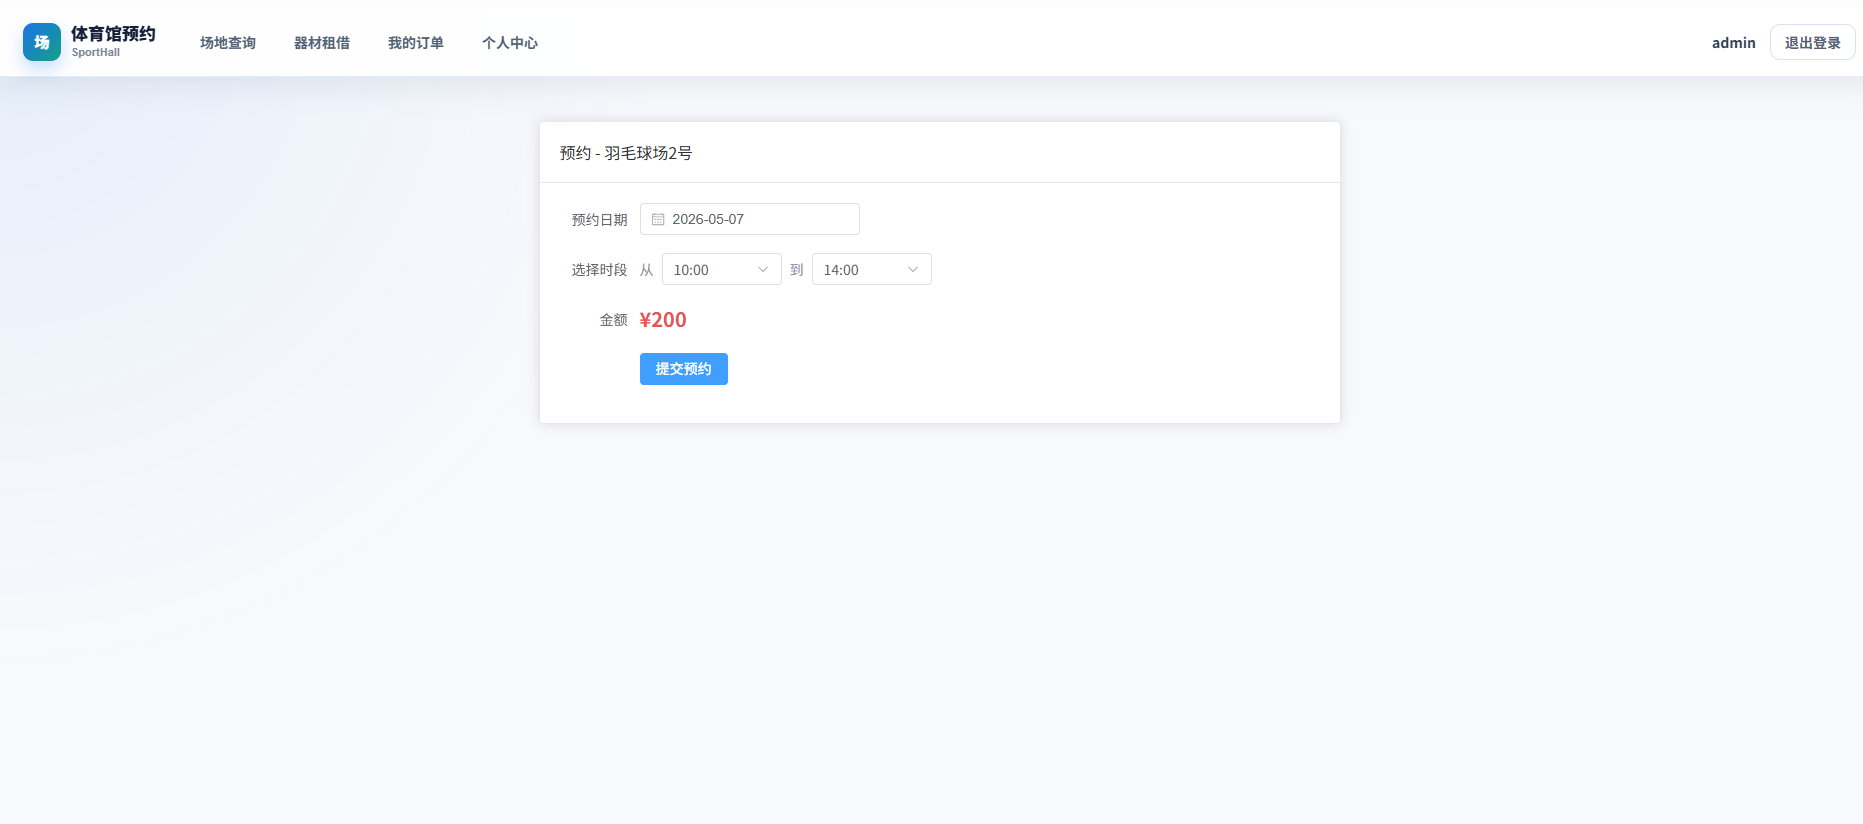
\includegraphics[width=0.8\textwidth]{img/fig5-2.png}
\caption{预约时段选择与下单页面}
\label{fig:booking-ui}
\end{figure}

\section{订单列表与状态操作实现}

订单列表页是对用户自己预约记录的展示页面。前端通过 /api/orders 获取分页信息，表格上订单号、预约时间、预约时间段、金额、状态都显示出来。系统把订单状态分为待支付、已支付和已取消三类，根据状态来决定是显示还是不显示支付和取消的操作。用户完成预约之后就会进入到个人订单页面，方便用户立即处理刚产生出来的待支付订单。

订单状态操作的限制只在后端。支付接口、取消接口都通过订单编号去查询记录，判断该订单是否是当前登录用户的所有订单，同时判断该订单的状态是否还为待支付。只有待支付订单才能变成已支付或者已取消状态，已经完成或者已经取消的订单不能再进行操作。因此即使前端页面没有立即刷新，后端也会阻止不合理的状态改变。

\begin{figure}[htbp]
\centering
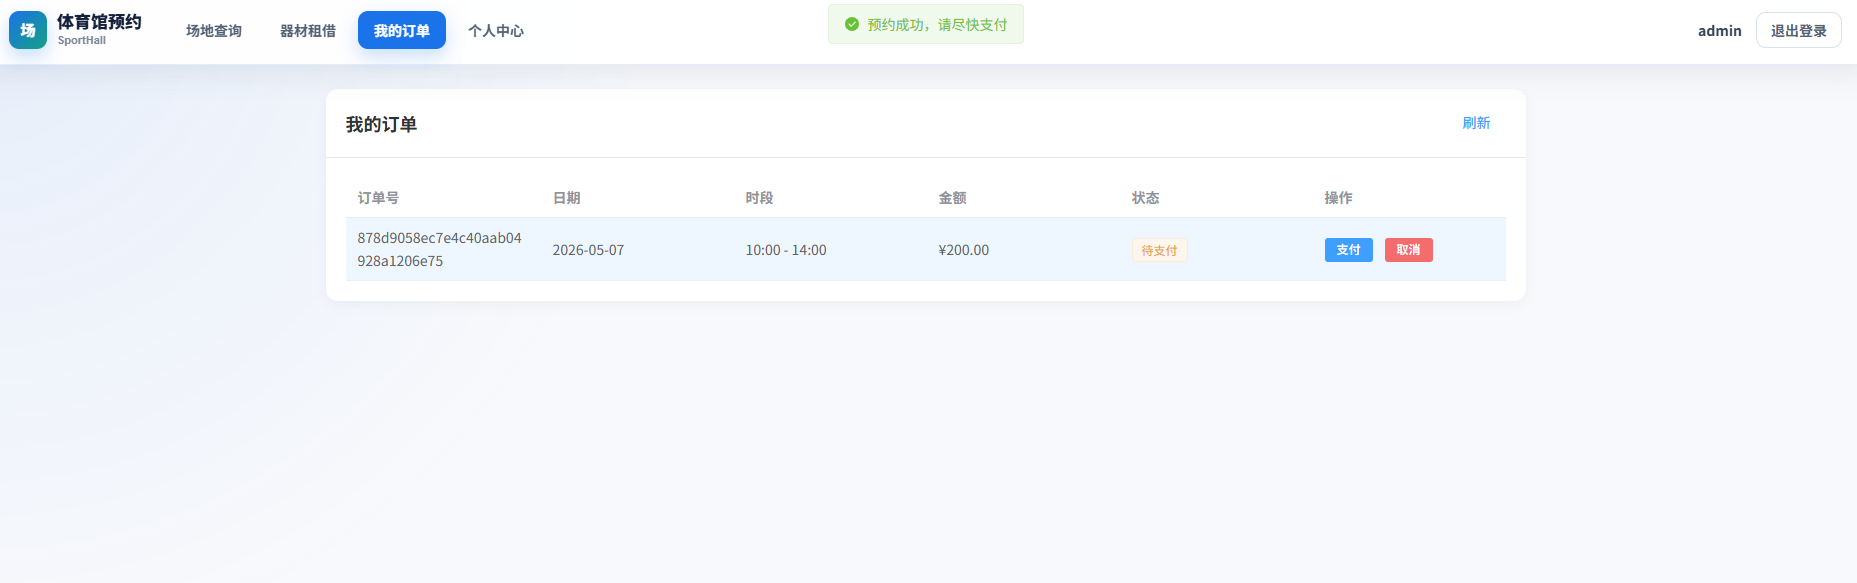
\includegraphics[width=0.8\textwidth]{img/fig5-3.png}
\caption{订单列表与状态操作页面}
\label{fig:order-ui}
\end{figure}

\section{器材租借与记录查询实现}

器材租借功能比场地预约流程短，但是要对库存一致性有要求。用户端器材页用 /api/equipments 获取器材列表，页面显示器材名称、总数量、可借数量和租借单价。用户输入数量之后提交租借申请，前端会对数量进行判断，数量大于 0 且不超过页面显示的可以借的数量；后端在设备服务中根据最新的库存重新验证，防止用户通过页面绕过或者在库存变化的时候提交已经过期的数据。

租借成功之后，后端会先从器材表里扣除可用量，然后写入一条租借记录，记录的状态为“租借中”。归还操作是由管理员来完成的，接口会根据租借记录编号去查找到原始的记录信息，看是否还在被占用的状态里。只有确认是原来的记录时，才可以对它进行增补操作，将其可借数量增加到原有的数字中来，并且把归还的时间写进去。租借、归还均在事务方法中完成，目的在于避免只对库存做了修改或者只对租借信息进行了更改而造成的中间状态。

\begin{figure}[htbp]
\centering
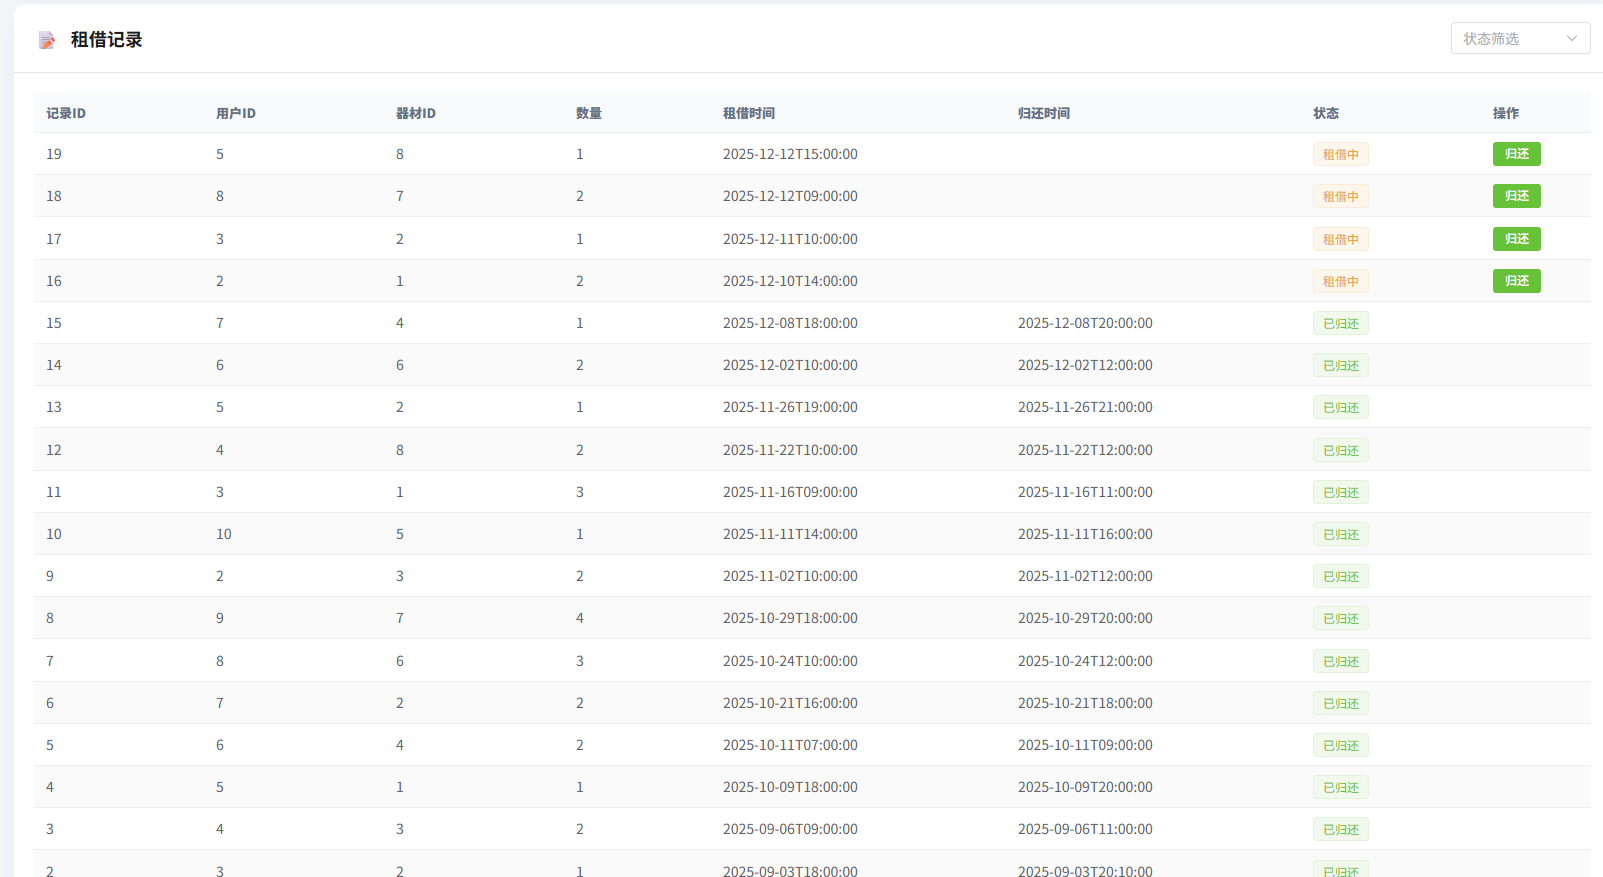
\includegraphics[width=0.8\textwidth]{img/fig5-4.png}
\caption{器材租借与记录查询页面}
\label{fig:equipment-ui}
\end{figure}

\section{场地管理页面实现}

场地管理页给管理员提供对场地基本资料的维护。页面主要是由表格和弹窗表单组成的，表格中显示场地名称、类型、开放时间、单价、状态；新增和修改都使用同一个表单，在编辑时会把当前行的数据带入到表单当中。上下架的操作单独设置为状态开关，在状态开关的上部可以自由调节场地开放状态，不需要打开编辑弹窗就可完成上下架操作。

后台对场地维护接口进行了管理员角色判断，普通用户即使知道接口地址也不能新增或者修改场地。新增或者修改的时候，系统会对名称、类型、开放时间、价格等进行校验，开放开始时间必须早于结束时间，价格不得小于 0。由于用户端预约页的生成可选时段会用到场地开放时间，因此这些校验直接会影响到后面预约流程能否进行。

\begin{figure}[htbp]
\centering
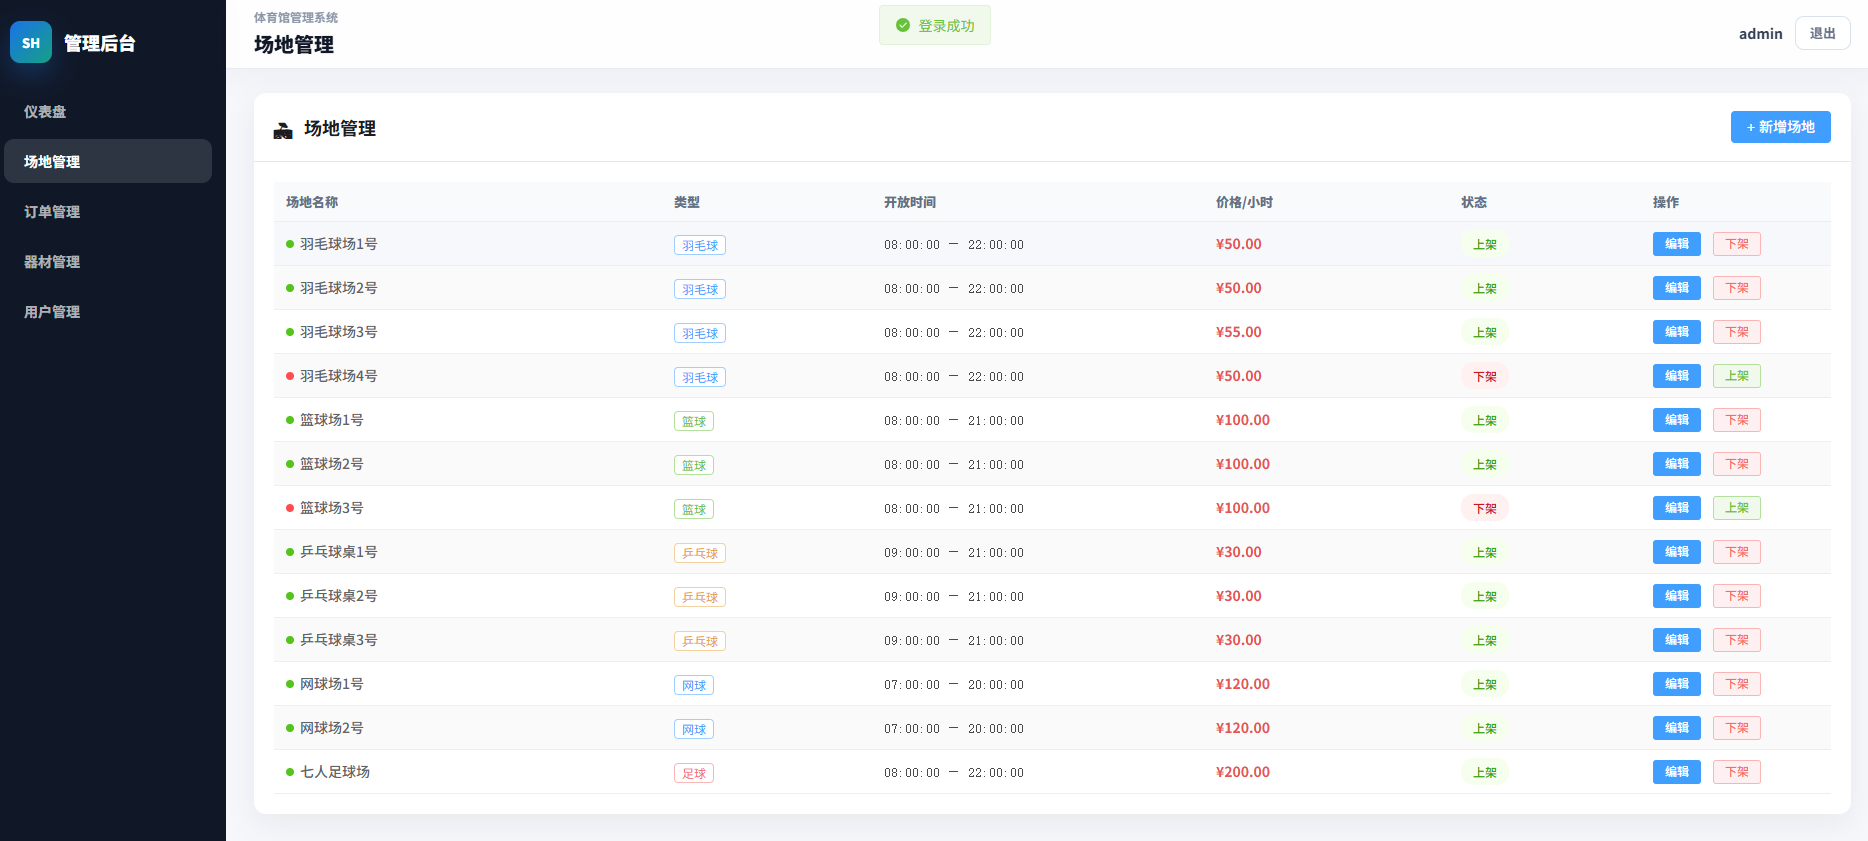
\includegraphics[width=0.8\textwidth]{img/fig5-5.png}
\caption{场地管理页面}
\label{fig:admin-venue-ui}
\end{figure}

\section{订单与用户管理实现}

后台订单管理页是管理员查看系统内所有的预约记录的界面。相比用户订单页来说，后台查询没有被限定当前用户编号的范围，按照订单状态和分页条件返回数据。该页面主要是实现对于已经支付的订单进行查询、对于已经取消的订单进行查询，以及对于近期预约的查询功能。由于本系统目前还没有接入真实的支付平台，支付操作仍然通过系统内部的状态变化来模拟，所以后台订单管理更多的是起到查询、核对的作用。

用户管理页是对注册的用户进行查看和角色调整。系统中的角色分为普通用户、管理员两种，前端路由会根据本地保存的角色信息来控制后台入口，但是真正的权限边界还在后台接口上。管理接口调用之前会先判断 JWT 中是否有 admin 这个角色，没有就拒绝处理。该种方式可以避免只依靠前端路由产生越权访问情况。

\begin{figure}[htbp]
\centering
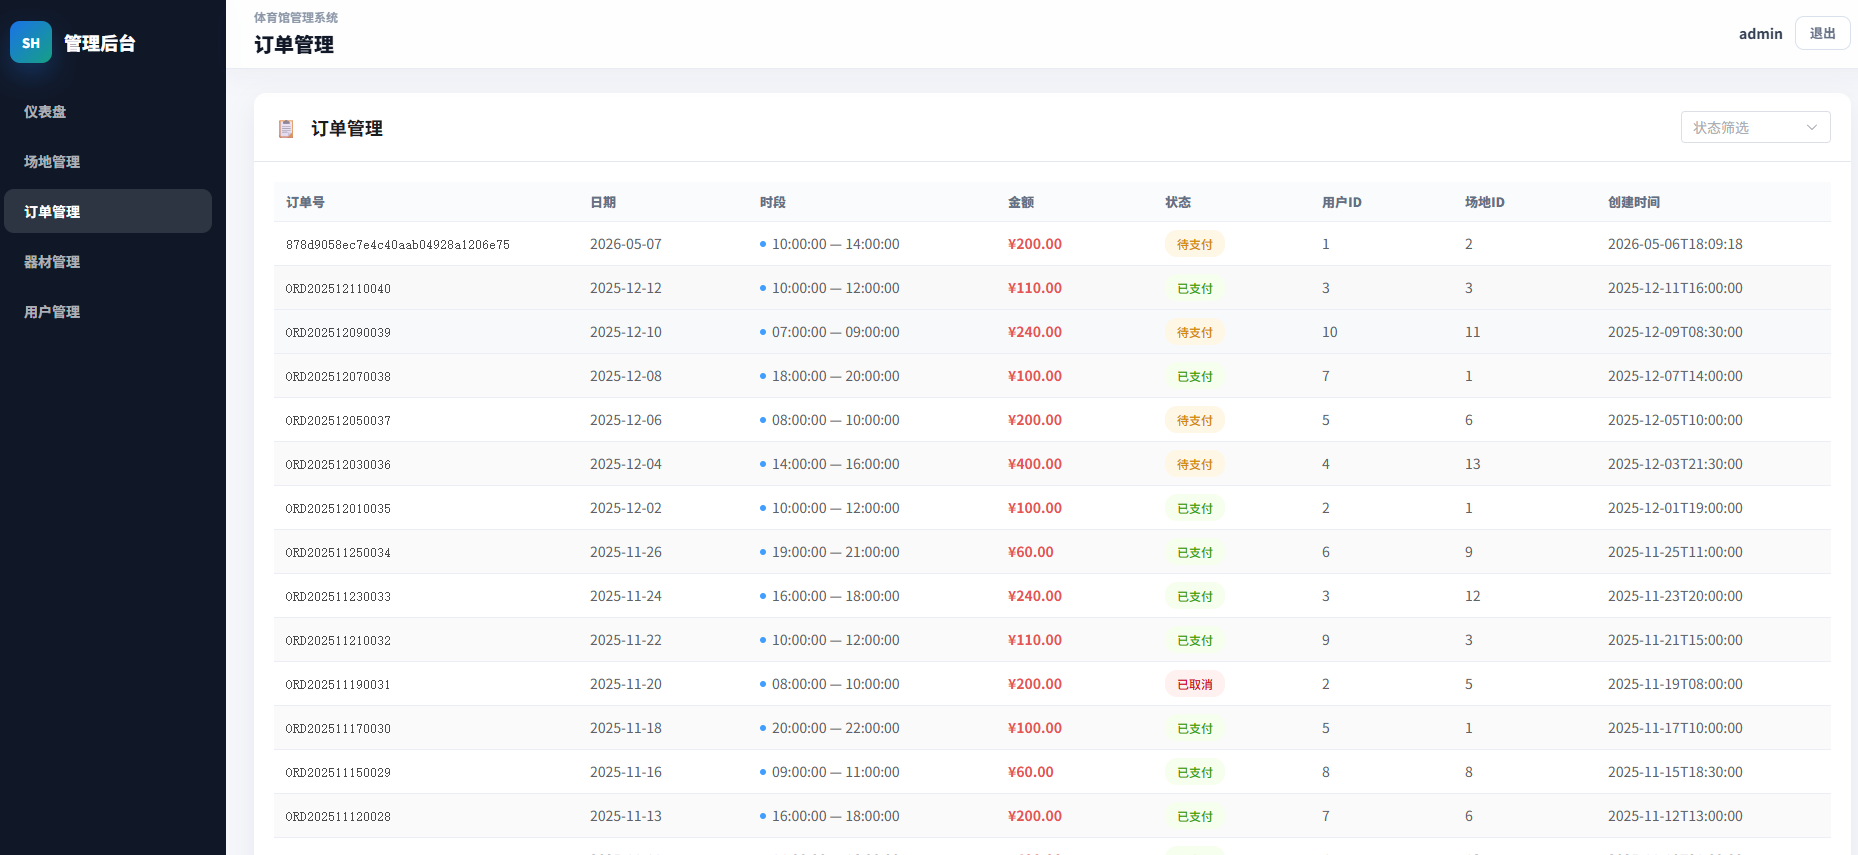
\includegraphics[width=0.8\textwidth]{img/fig5-6.png}
\caption{订单管理页面}
\label{fig:admin-order-ui}
\end{figure}

\begin{figure}[htbp]
\centering
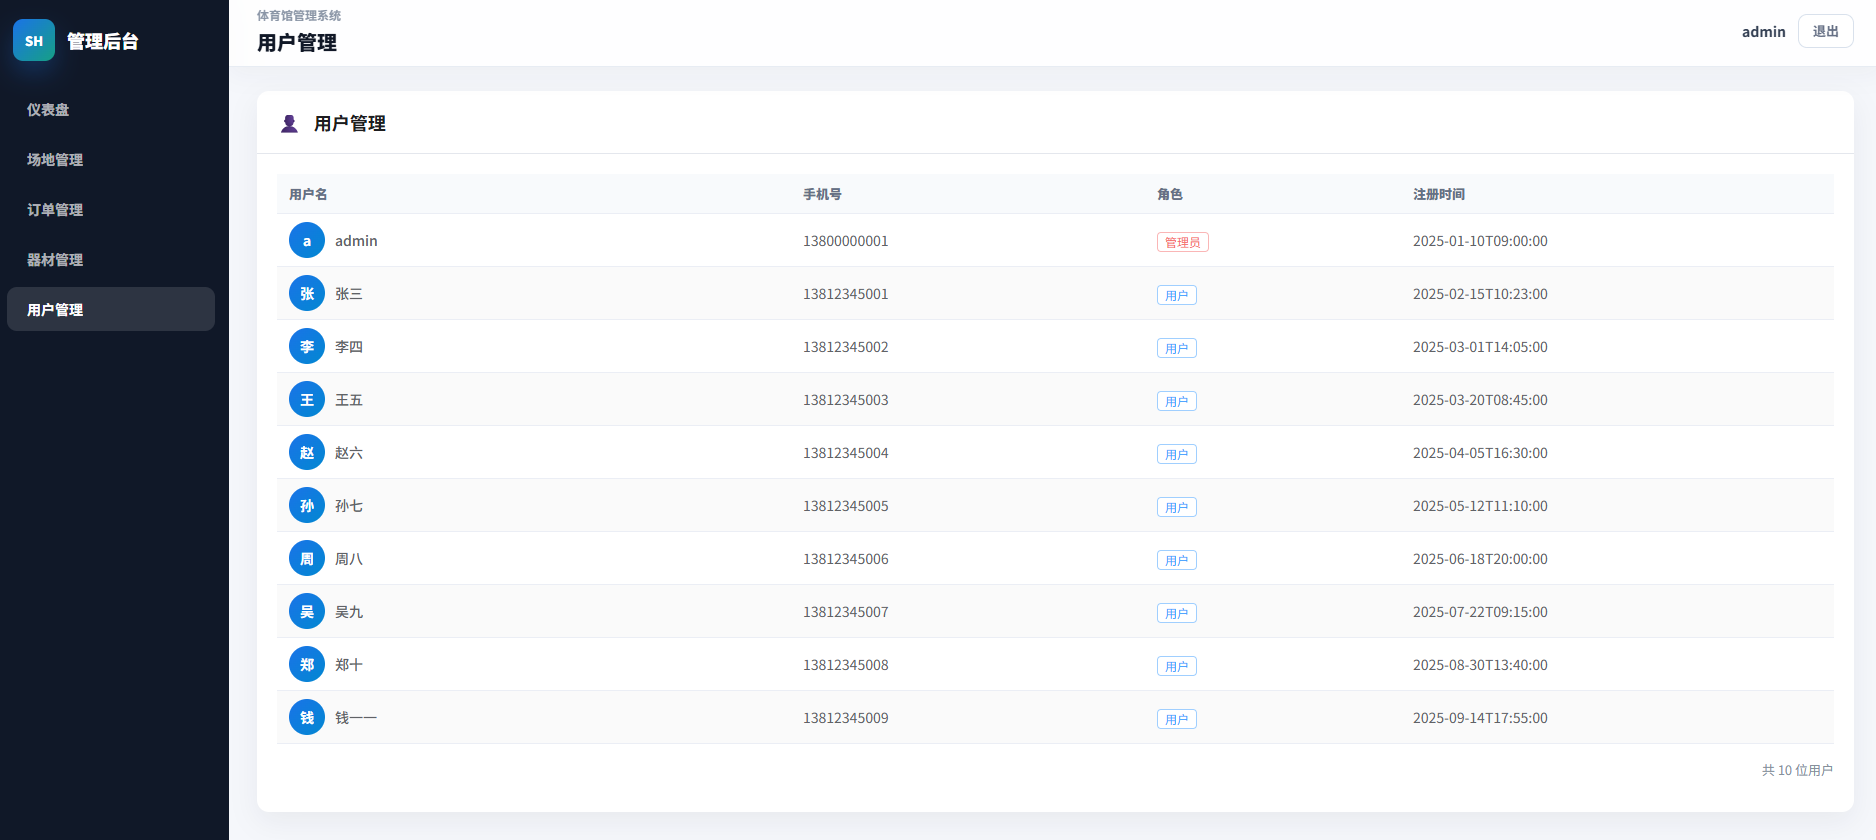
\includegraphics[width=0.8\textwidth]{img/fig5-7.png}
\caption{用户管理页面}
\label{fig:admin-user-ui}
\end{figure}

\section{器材信息维护实现}

器材信息维护页用来管理器材名称、总数量、可借数量、租借单价。新增器材时，如果管理员没有单独填写可借数量，系统默认可借数量为总数量；修改器材时，系统不能简单地覆盖库存，因为已经存在的尚未归还的租借记录会受到影响。后台先求出已有借出的数量，再判断新的总数小于已借出的多少个。新总的大小太小了，接口就会拒绝更新，不能出现可以借的量为负数的情况。

这部分逻辑放到后端实现，主要是因为前端页面只能体现打开页面时的数据状态，库存会随着用户租借或者管理员归还发生变化。后端更新时重新读取数据库中旧的记录，可以减少库存计算使用过期页面数据的问题。

\begin{figure}[htbp]
\centering
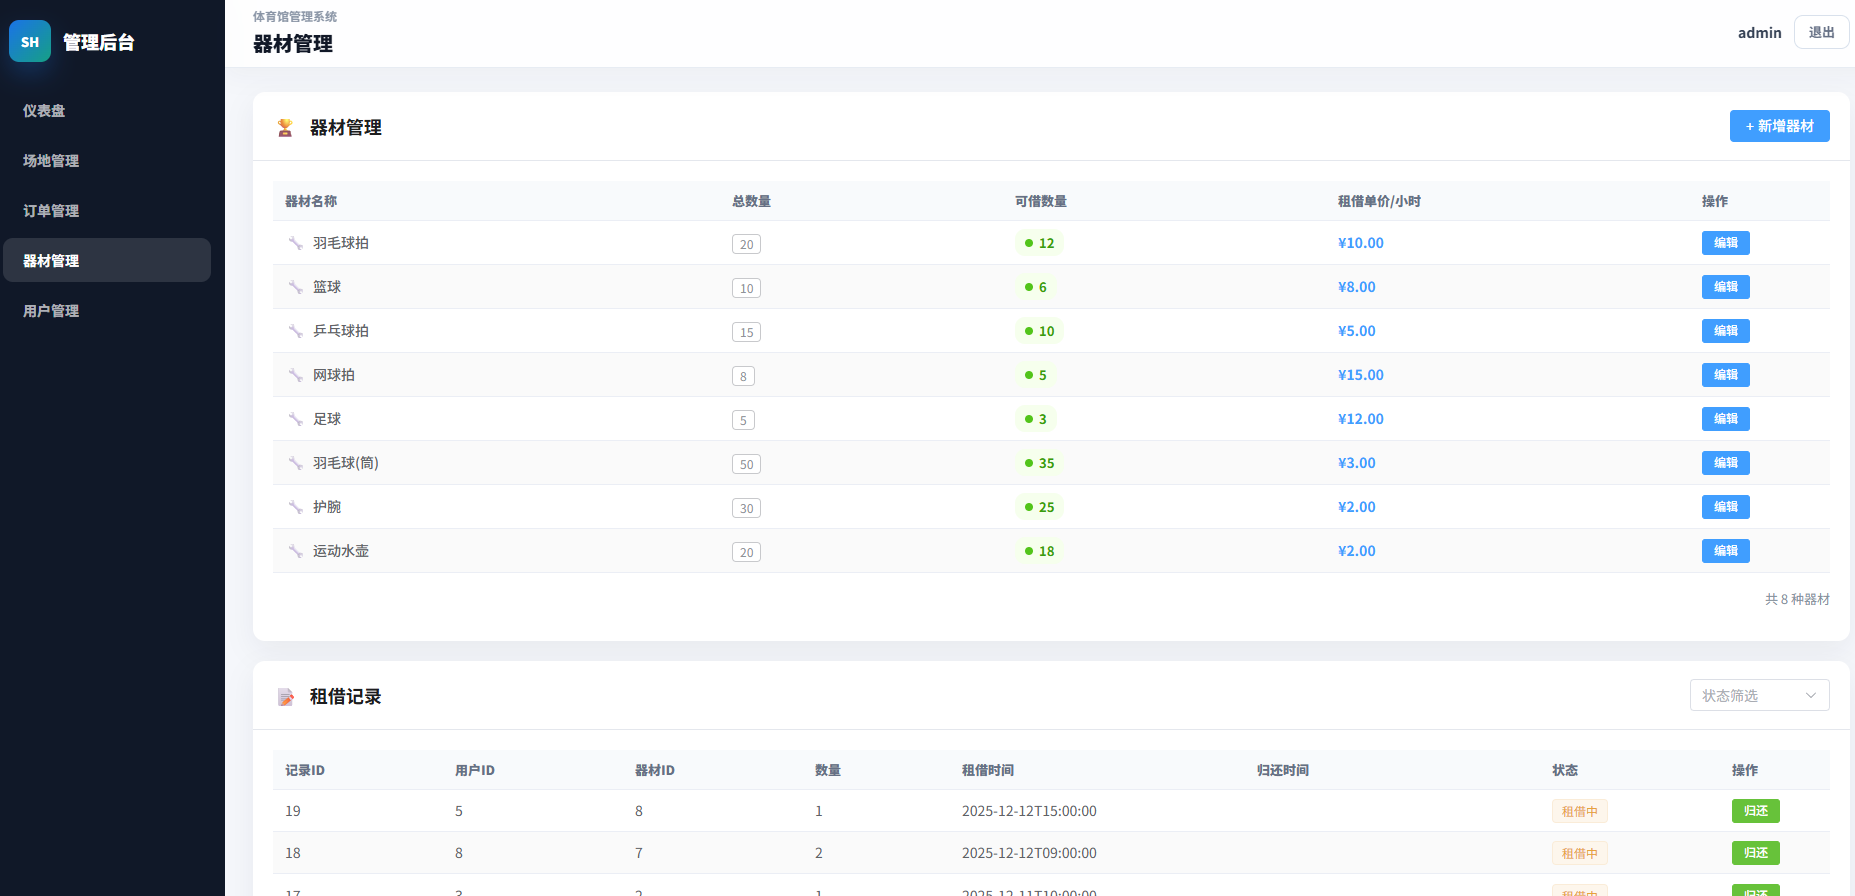
\includegraphics[width=0.8\textwidth]{img/fig5-8.png}
\caption{器材信息维护页面}
\label{fig:admin-equipment-ui}
\end{figure}

\section{数据统计看板实现}

后台首页的数据看板是给管理员提供的一个快捷的入口。页面加载的时候同时请求场地、订单、器材、用户相关接口，在前端计算出开放场地数、订单总量、已支付订单数、器材总库存、可借库存、注册用户数量等指标。页面会以近 7 日为单位，用简单的柱状图展示最近的订单情况以及最近的预约日期。由于本系统数据量小，可以全部在前端进行统计，代码也较易理解。

需要指出的是，目前的看板还只是基础统计，并没有单独设计出统计表或者复杂的图表接口。当后期订单数量增多时，前端仍然从后端拉取过多的订单再进行计算是不可取的，应该改为后端提供聚合接口，例如按日期统计订单数量、按场地类型统计使用率等。本课题现阶段保留简单的实现是为了满足管理员查看系统运行情况的需求。

\begin{figure}[htbp]
\centering
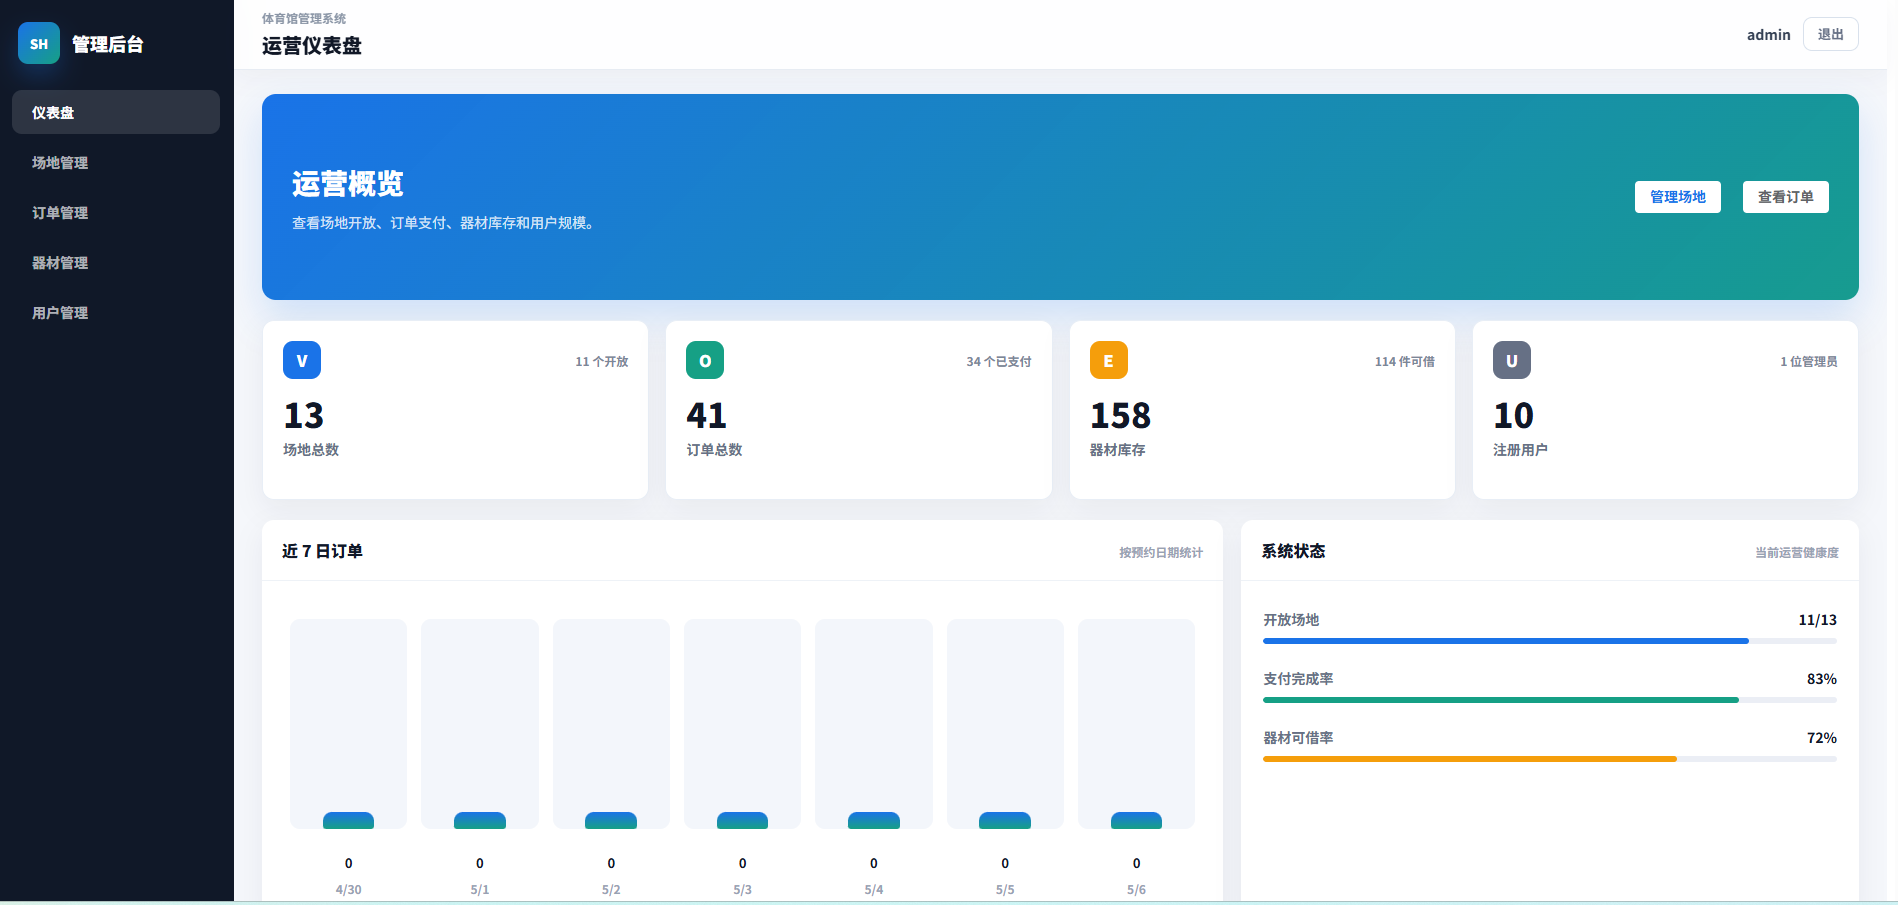
\includegraphics[width=0.8\textwidth]{img/fig5-9.png}
\caption{数据统计看板页面}
\label{fig:dashboard-ui}
\end{figure}
